\section{Application to SimSoC-cert}
\label{sec:simsoccert}

SimSoC-Cert~\cite{rapido11,cpp11} aims at certifying the simulator SimSoC, 
which is a complex hardware simulator written in C and C++.
SimSoC is able to simulate ARM and PowerPC architectures and is 
efficient enough to run Linux on both of them at a realistic speed.
The main objective of SimSoC is to help designers of embedded systems:
a large part of the design can be performed on software,
which is is much more convenient, flexible and less expensive
than with real specific hardware components.
However, 
this only makes sense if the simulator is actually faithful to the real
hardware.
Therefore we engaged in an effort to provide a formal certification
of sensitive parts of SimSoC.
More precisely, we consider the Instruction Set Simulator (ISS)
for the ARM, which is at the heart of SimSoC.
This ISS is called Simlight.

To this effect, we provide first defined a formal model in Coq of the ARM
architecture, as defined in the reference manual.
This is essential for defining the reference expected behavior
of SimSoC.
Our second input is the operational semantics of the ISS
encoded in C. 
This program is actually written in a large enough subset of C
called Compcert-C,
which is fully formalized in Coq \cite{Leroy-Compcert-CACM}.

We can then compare the behavior of the ISS encoded in C 
with the expected reference model directly defined in Coq.
To this effect, a projection between the Coq model of the
memory state of Simlight to the states in the reference model
is defined.
Then, correctness statements express that from a 
C memory $m_1$ corresponding to an abstract state $s_1$,
performing the function claimed to represent a given instruction $\cal I$
in Simlight 
will result in a C memory $m_2$ which actually corresponds 
to the abstract state $s_2$ obtained by
running the Coq model of $\cal I$. 
This can be put under the form of a commutative diagram as
schematized in Fig.~\ref{fig:thrm}.
%% HERE THE FIGURE 

\begin{figure}
\hfil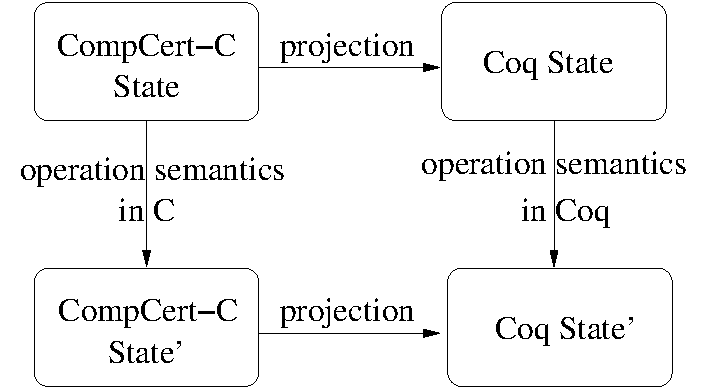
\includegraphics[width=.5\linewidth]{theorem.pdf}
\caption{Correctness of the simulation of an ARM operation}
\label{fig:thrm}
\end{figure}

In details,
changes in the C memory model are formally described
by a transition system according to the operational semantics of Compcert-C.
Therefore, the later is used everywhere in the proofs. 
This operational semantics is described by
a big mutual inductive type;
in particular, the evaluation of expressions is defined by
16 constructors, one for each CompCert C expression like assignment or binary
operation.
% And this inductive type evaluation of expression is our target to try the
% improved new inversion.
A typical proof step start from a goal intuitively saying that,
given two C memory states related by a C expression,
as expressed in some hypothesis $H$, 
some commutative diagram holds.
Then $H$ is inverted, which either yields more elementary 
transitions between C memory states, 
with corresponding expected commutative diagrams,
or solves the current diagram if the considered expression
is atomic. 
In general we see that an inversion will result in many
new opportunities to perform inversions.

In our first proofs, using the Coq standard \inversion tactic
resulted in a very weak control on the script.
Finding the right relation to focus on in the hypotheses
was inconvenient.
Interactive execution of the script was also quite slow,
due to the size of the terms generated by \inversion.
And the compilation time for the proof on only one instruction 
took more than one minute --
there are more than one hundred instructions in the ARMv6 architecture.
Moreover
the proof code is fragile in case of changes: 
after \inversion, hypotheses are automatically given similar names 
according to a simple numbering scheme,
so that any modification at the beginning of the proof script
or in auxiliary lemmas 
result in a complete renaming of hypotheses to come in the sequel.
This is quite harmful in practice and constitutes
a serious issue for maintenance.

The following code shows an small excerpt from 
an old proof script in SimSoC-Cert using \inversion.
In this example, we want to find out the relation between memory states
\coqdocvar{m} and \coqdocvar{m'} expressed in the hypothesis $H$,
whose main argument (\coqdocvar{Ecall (Evalof...})
represents the program to be executed.
Its type is given by the inductive relation \coqdocvar{eval\_expr}.
%To achieve this goal, we use \inversion step
%following step by step the definition of semantics of \coqdocvar{eval\_expr}.
We see that many \coqdocvar{inv Hx} are used.
Here \coqdocvar{inv H} denotes \coqdocvar{inversion H; clear H; subst}.

\medskip
\dots \\
\coqdocinput{chunk41}

\coqdocinput{chunk42}
\dots
\medskip

The program for simulating an ARM instruction 
usually contains expressions more complex than in the
example given here.
% We have to invert the predicate so many times to find the relation between
% initial and final memory state. 
This cumbersome work is needed in every instruction proofs,
and there is no clear way to share anything since
the corresponding programs are rather specific,
at least for instructions belonging to different categories.

Thanks to the technique introduced in this paper,
we could define convenient reusable tactics.
First, we defined suitable diagonal-based functions for each
constructor of $eval\_expr$ following the lines given in the
previous section.
Then we packaged them altogether in a high-level tactic named 
$inv\_eval\_expr$ using a Ltac definition. The arguments of this
tactic are the memory states under focus --
in the example above: $m$ and $m'$.
This tactic also contains extra features so that
it is able to:
%
\begin{enumerate}
\item find automatically an hypothesis to be inverted;
\item repeatedly perform our hand-crafted inversion until all constraints
  between two memory state are derived;
\item give meaningful names to the derived constraints;
\item update all other related hypotheses according to the new 
  variables names or values;
\item clean up useless variables and hypotheses.
\end{enumerate}
%
Then all the eighteen \inversion in the example above are solved in just
one step using $inv\_eval\_expr m m'$.

To be fair, let us mention that the robustness issue could,
in principle, be managed using the current version of standard \inversion,
because of allows us 
to give explicit names to introduced variables and hypotheses.
However, due to the complexity of CompCert C semantics, 
providing all these names explicitly turns out to be cumbersome,
and unrealistic when you face dozens of consecutive \inversion 
and about ten names for each \inversion.
Within our framework,
the introduction suitable names 
is automatically performed inside $inv\_eval\_expr m m'$.
Names are chosen according to the contents and in a flexible way, 
so that the evolution of goals is easy to follow.

As a unexpected benchmark, 
when CompCert C semantics has been changed to a new version
in the end of 2011,
we didn't have to change the proofs:
just updating the tactic turned out to be enough. 

Comparing development times is provides additional hints.
In our first try, dedicated to the instruction ADC,
more than two months were spent on the development of the correctness proof.
The inversion technique presented here was not available
at that time, entailing the drawbacks detailed above.
With the new approach, proofs for 4  other instructions
could be finished in only one week. 
The high-level tactic described above required
less than 2 weeks.


Finally, 
we compare the efficiency of the standard Coq \inversion with our new tactic
in Table.~\ref{t:timing}.
The first line is about the whole expression given in the example above. 
The other lines are inversions of specific expressions.
We can observe a gain of about 4 to 5 times.

\begin{table}\centering
\label{t:timing}
\caption{Comparison of the time costs}
\begin{tabular}{|l|c|c|}
\hline
 & standard \inversion & our inversion \\
\hline
Full example &  1.856& 0.404\\
\hline
Ebinop & 0.104&  0.020\\
\hline
Evalof &  0.096& 0.020\\
\hline
Eval &  0.116& 0.020\\
\hline
Evar &  0.108& 0.024\\
\hline
\end{tabular}
\end{table}



%%% Local Variables: 
%%% mode: latex
%%% TeX-master: "cpp12"
%%% End: 
